\chapter{Marktumgebung}

\section{Kundenseitige Entwicklungen}

Da die Preise für die europäischen Emissionszertifikate (EU-ETS) -- gegeben innereuropäisch bleiben die politischen Verhältnisse vergleichsweise stabil -- in naher Zukunft steigen werden und positive Nettoemissionen letztendlich in weiten Teilen vollständig verboten werden, wird es für Kunden stetig attraktiver, ihr Nettoemissionsprofil zu reduzieren und so ihre Wirtschaftlichkeit zu erhalten oder gar zu erhöhen.
% Gegebenenfalls nochmal umformulieren
Insbesondere für jene Sektoren mit besonders intensiven Emissionen oder solche, deren Geschäftsmodel inhärent keine weitere Verbesserung ihrer CO2-Bilanz zulässt wird es um das ökonomische Überleben gehen.

Ab Februar 2024 werden die Emissionszertifikate je Tonne CO2 mit \qty{68}{\EUR} bewertet (siehe \cref{fig:carbon price tracker}), wobei die Bepreisung der Kombination aus Marktdynamik und regulatorischen Änderungen unterliegt.
Im mittel und langfristigen Trend wird hier mit einem stetigen Anstieg der Kosten für Emissionszertifikate zu rechnen sein und spiegelt das Engagement der EU zur Erreichung ihrer Klimaziele wider.

\begin{figure}[h]
    \centering
    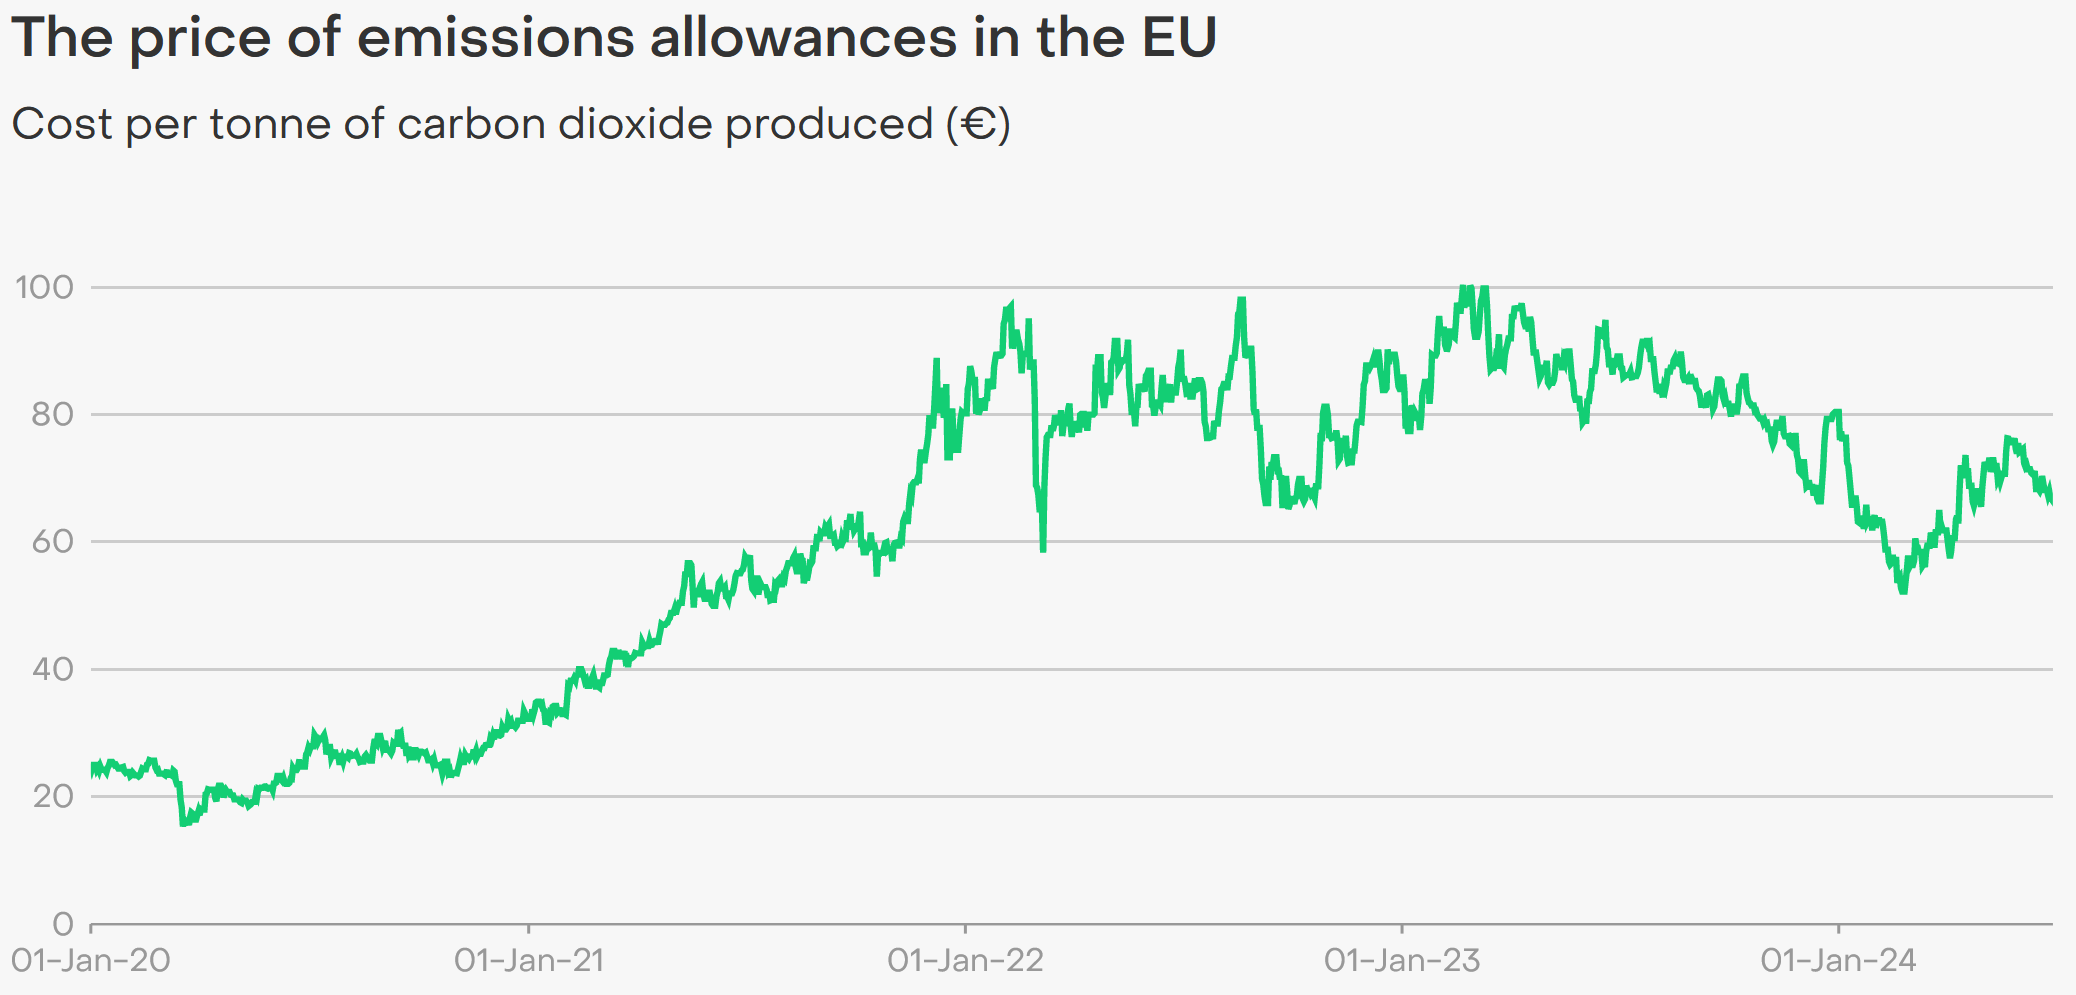
\includegraphics[width=.9\textwidth]{Carbon Price Tracker_Ember.png}
    \caption[Entwicklung der CO2-Bepreisung in der EU]{Entwicklung der CO2-Bepreisung in der EU von 2020 bis heute.}\label{fig:carbon price tracker}
\end{figure}

Strengere Klimapolitik und sinkende Obergrenzen für die Gesamtemissionen reduzieren darüber hinaus die am Markt verfügbaren Emissionszertifikate um -- nach aktueller Rechtslage -- spätestens im Jahr 2045 bei defacto null zu sein.
% Das regulatorische Umfeld wird immer strenger, und es wird erwartet, dass Nettoemissionen in naher Zukunft gänzlich verboten werden.
Regulatorischer Druck zwingt die Unternehmen dazu, nach innovativen Lösungen zu suchen, um ihren Kohlenstoff-Fußabdruck zu verringern und so langfristig rentabel wirtschaften zu können.

Die Notwendigkeit CO2-neutral zu wirtschaften durchdringt auch immer weiter in die allgemeine Gesellschaft vor was sich etwa im Konsumverhalten widerspiegelt.
Ein klimafreundliches Image wird für Unternehmen folglich zunehmend wichtiger um sich am Markt positiv hervortun zu können.\par\medskip
% In Anbetracht der steigenden Kosten für Emissionszertifikate und der sich verschärfenden rechtlichen Rahmenbedingungen können die Kunden erhebliche finanzielle Vorteile aus Investitionen in Technologien ziehen, die ihr Nettoemissionsprofil reduzieren.

Vorteile durch den Einsatz von \textsc{Green Wall}s fortschrittlichen Carbon Capture and Storage/Utilization (CCS/U) Systemen:

\begin{itemize}
    \item Reduktion von Ausgaben: Abhängigkeit von Emissionszertifikaten reduzieren durch Verringerung ihrer Netto-CO2-Emissionen.
    \item Rentabilität: Abfedern der finanziellen Auswirkungen steigender Preise für Emissionszertifikate.
    \item Compliance: Sicherstellung der Einhaltung aktueller und zukünftiger gesetzlicher Vorschriften, Vermeidung von Strafen und Verbesserung der Außendarstellung des Unternehmens.
    \item Nachhaltige Praktiken: Demonstration des eigenen Engagements für nachhaltiges Wirtschaften, was wiederum den Markenwert steigern und umweltbewusste Kunden und Investoren anziehen kann.
\end{itemize}

Die steigenden Kosten für Emissionszertifikate und das drohende Verbot positiver Netto-Emissionen eröffnen einen neuen Markt für innovative CCS/U-Lösungen: Unternehmen aus unterschiedlichen Sektoren, darunter die verarbeitende Industrie, der Energiesektor und die Landwirtschaft suchen aktiv nach kostengünstigen und effizienten Lösungen, um ihren Kohlenstoff-Fußabdruck zu verringern.
\textsc{Green Wall}s modulare Mikroalgen-Bioreaktoren bieten eine skalierbare und vielseitige Lösung, die diesen Anforderungen gerecht wird.\par\medskip

Weltweit verzeichnet das Produktionsvolumen von Biokraftstoffen einen nahezu exponentielles Wachstum.
In \cref{fig:biofuel production} zu sehen ist das deutsche Produktionspotenzial noch nicht vollständig ausgeschöpft. 
Neben der aktiven Entnahme von Kohlenstoffdioxid aus der Luft durch \textsc{Green Wall}s Bioreaktoren kann das in den Bioabfällen gebundene CO2 als lokal produzierter und hochpotenter Rohstoff für die Biotreibstoffherstellung genutzt werden.
% Durch die Positionierung als führendes Unternehmen im Bereich des Biotechnologiebasierten CCS/U ist \textsc{Green Wall} an der Spitze der Transformation von Industrien und Staaten hin zu einer CO2-neutralen und nachhaltigen Wirtschaft auch dort, wo auf CO2-Emissionen nicht verzichtet werden kann.

\textsc{Green Wall}s Portfolio erfüllt nicht nur die unmittelbaren Bedürfnisse seiner Kunden, sondern bietet auch langfristige Wettbewerbsvorteile, indem sie zu einer nachhaltigen und kohlenstoffneutralen Zukunft beiträgt.

\begin{figure}[h]
    \centering
    \includesvg[width=.9\textwidth]{biofuel_prod}
    \caption[Entwicklung des Produktionsvolumens von Biotreibstoff]{Entwicklung des Produktionsvolumens von Biotreibstoff.}\label{fig:biofuel production}
\end{figure}